\documentclass[11pt,a4j]{jreport}
\title{レポートフォーマットについて}
\author{マク}
\date{2019 /8/13}
\usepackage{booktabs}
\usepackage[dvipdfmx,hiresbb]{graphicx}
%\pagestyle{empty}
\renewcommand{\bibname}{参考文献} % [thebibliography] 関連図書 ==> 参考文献

% 数式番号にsectionを付加
\makeatletter
\@addtoreset{equation}{section}
\def\theequation{\thesection.\arabic{equation}}
\makeatother

\begin{document}

 
% 目次
{\makeatletter
\let\ps@jpl@in\ps@empty
\makeatother
\pagestyle{empty}
\tableofcontents
\clearpage}

% Chapter1
\setcounter{page}{1} % 本文からページ番号を振りはじめる  
\pagestyle{plain}
 \chapter{序論}
章テスト\cite{bunshun}

 \begin{figure}[htbp]
  \centering
  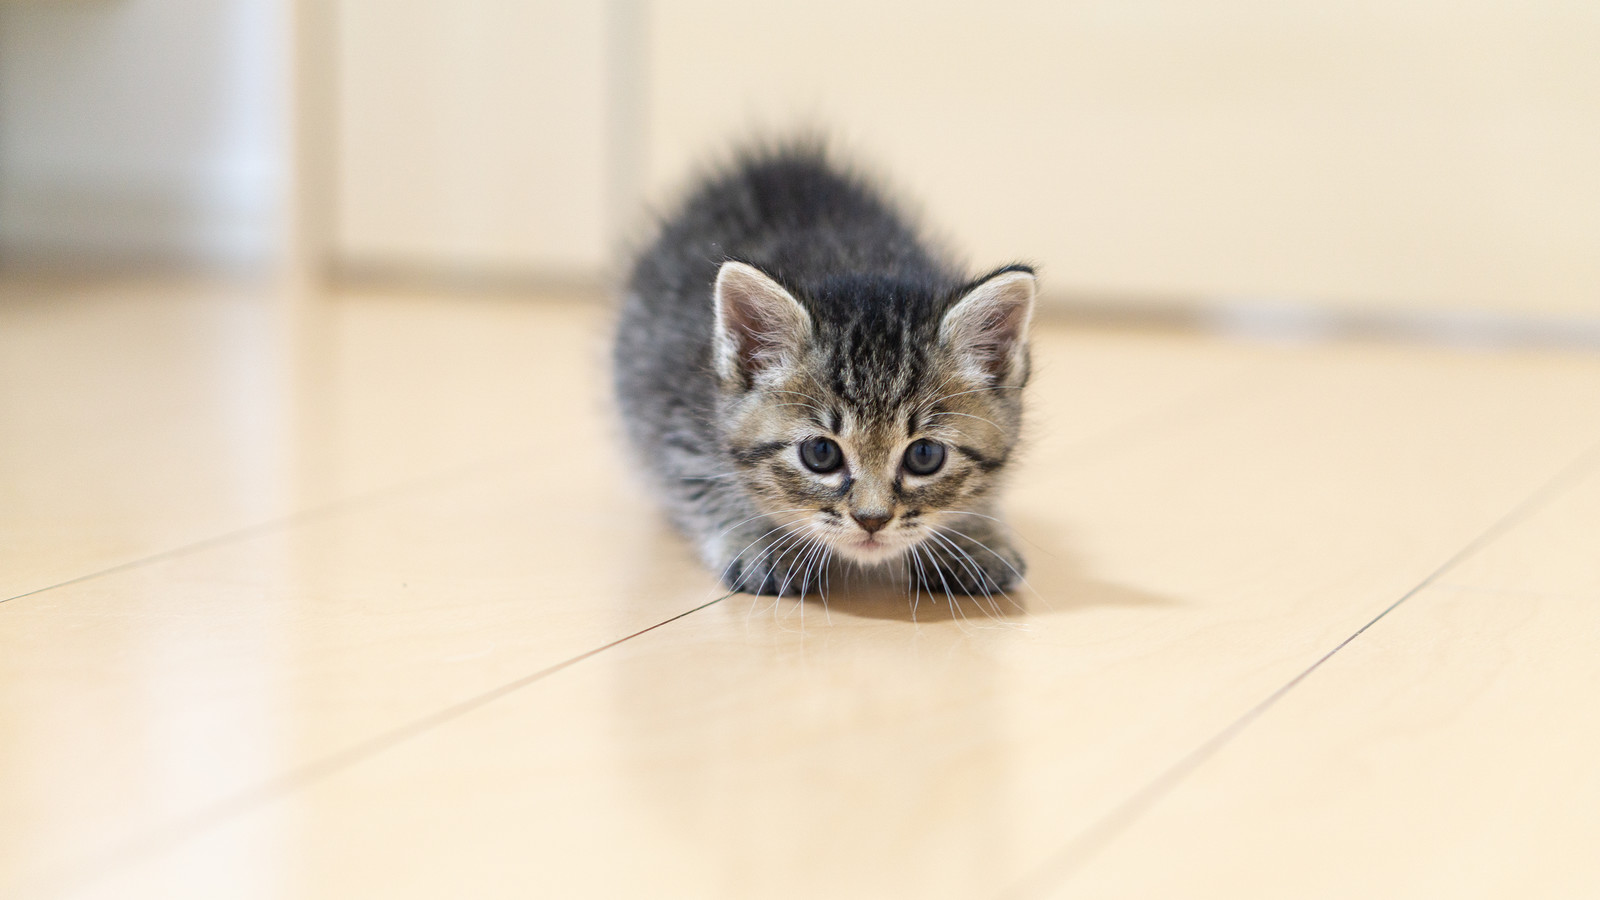
\includegraphics[width=14cm,clip]{image/TOMS526509_TP_V.jpg}
  \caption{猫の画像\cite{cat-src}}
  \label{cat}
 \end{figure}
 
 
  \begin{table}[htb]
  \begin{center}
    \caption{各商品の値段と個数}
    \begin{tabular}{lcc} \toprule
商品名 & 個数/個 & 値段/円 \\ \midrule
バナナ & 3 & 300 \\
梨 & 4 & 500 \\ \bottomrule
    \end{tabular}
    \label{shop}
  \end{center}
 \end{table}

  % 節
  \section{節}
  節テスト(図\ref{cat}.参照)
  
    % 項
    \subsection{項}
    項テスト
  
% Chapter2
 \chapter{結論}
  
  \section{結論}

  \section{今後の展望} 
  
  
% 参考文献
 \begin{thebibliography}{99}
  \bibitem{bunshun}イアン・エアーズ.その数学が戦略を決める.文春文庫
  \bibitem{cat-src}"身構えてもかわいい子猫".無料の写真素材はフリー素材のぱたくそ.https://www.pakutaso.com/20190618179post-21118.html
 \end{thebibliography} 
  
% 謝辞
 \chapter*{謝辞}
  
  
\end{document}
